%%%%%%%%%%%%%%%%%%%%%%%%%%%%%%%%%%%%%%%%%
% Arsclassica Article
% LaTeX Template
% Version 1.1 (1/8/17)
%
% This template has been downloaded from:
% http://www.LaTeXTemplates.com
%
% Original author:
% Lorenzo Pantieri (http://www.lorenzopantieri.net) with extensive modifications by:
% Vel (vel@latextemplates.com)
%
% License:
% CC BY-NC-SA 3.0 (http://creativecommons.org/licenses/by-nc-sa/3.0/)
%
%%%%%%%%%%%%%%%%%%%%%%%%%%%%%%%%%%%%%%%%%

%----------------------------------------------------------------------------------------
%	PACKAGES AND OTHER DOCUMENT CONFIGURATIONS
%----------------------------------------------------------------------------------------

\documentclass[
12pt, % Main document font size
a4paper, % Paper type, use 'letterpaper' for US Letter paper
oneside, % One page layout (no page indentation)
%twoside, % Two page layout (page indentation for binding and different headers)
headinclude,footinclude, % Extra spacing for the header and footer
BCOR5mm, % Binding correction
]{scrartcl}

%%%%%%%%%%%%%%%%%%%%%%%%%%%%%%%%%%%%%%%%%
% Arsclassica Article
% Structure Specification File
%
% This file has been downloaded from:
% http://www.LaTeXTemplates.com
%
% Original author:
% Lorenzo Pantieri (http://www.lorenzopantieri.net) with extensive modifications by:
% Vel (vel@latextemplates.com)
%
% License:
% CC BY-NC-SA 3.0 (http://creativecommons.org/licenses/by-nc-sa/3.0/)
%
%%%%%%%%%%%%%%%%%%%%%%%%%%%%%%%%%%%%%%%%%

%----------------------------------------------------------------------------------------
%	REQUIRED PACKAGES
%----------------------------------------------------------------------------------------

\usepackage[
nochapters, % Turn off chapters since this is an article        
beramono, % Use the Bera Mono font for monospaced text (\texttt)
eulermath,% Use the Euler font for mathematics
pdfspacing, % Makes use of pdftex’ letter spacing capabilities via the microtype package
dottedtoc % Dotted lines leading to the page numbers in the table of contents
]{classicthesis} % The layout is based on the Classic Thesis style

\usepackage{arsclassica} % Modifies the Classic Thesis package

\usepackage[T1]{fontenc} % Use 8-bit encoding that has 256 glyphs

\usepackage[utf8]{inputenc} % Required for including letters with accents

\usepackage{graphicx} % Required for including images
\graphicspath{{Figures/}} % Set the default folder for images

\usepackage{enumitem} % Required for manipulating the whitespace between and within lists

\usepackage{lipsum} % Used for inserting dummy 'Lorem ipsum' text into the template

\usepackage{subfig} % Required for creating figures with multiple parts (subfigures)

\usepackage{amsmath,amssymb,amsthm} % For including math equations, theorems, symbols, etc

\usepackage{varioref} % More descriptive referencing

\usepackage{listings}
%----------------------------------------------------------------------------------------
%	THEOREM STYLES
%---------------------------------------------------------------------------------------

\theoremstyle{definition} % Define theorem styles here based on the definition style (used for definitions and examples)
\newtheorem{definition}{Definition}

\theoremstyle{plain} % Define theorem styles here based on the plain style (used for theorems, lemmas, propositions)
\newtheorem{theorem}{Theorem}

\theoremstyle{remark} % Define theorem styles here based on the remark style (used for remarks and notes)

%----------------------------------------------------------------------------------------
%	HYPERLINKS
%---------------------------------------------------------------------------------------

\hypersetup{
%draft, % Uncomment to remove all links (useful for printing in black and white)
colorlinks=true, breaklinks=true, bookmarks=true,bookmarksnumbered,
urlcolor=webbrown, linkcolor=RoyalBlue, citecolor=webgreen, % Link colors
pdftitle={}, % PDF title
pdfauthor={\textcopyright}, % PDF Author
pdfsubject={}, % PDF Subject
pdfkeywords={}, % PDF Keywords
pdfcreator={pdfLaTeX}, % PDF Creator
pdfproducer={LaTeX with hyperref and ClassicThesis} % PDF producer
} % Include the structure.tex file which specified the document structure and layout

\hyphenation{Fortran hy-phen-ation} % Specify custom hyphenation points in words with dashes where you would like hyphenation to occur, or alternatively, don't put any dashes in a word to stop hyphenation altogether

%----------------------------------------------------------------------------------------
%	TITLE AND AUTHOR(S)
%----------------------------------------------------------------------------------------

\title{\normalfont\spacedallcaps{ERG3020 Report}} % The article title

%\subtitle{Subtitle} % Uncomment to display a subtitle

\author{\spacedlowsmallcaps{Zhuoyu Li\& Bokai Xu\& Xiyan Luo}} % The article author(s) - author affiliations need to be specified in the AUTHOR AFFILIATIONS block

\date{2021.5.5} % An optional date to appear under the author(s)

%----------------------------------------------------------------------------------------

\begin{document}

%----------------------------------------------------------------------------------------
%	HEADERS
%----------------------------------------------------------------------------------------

\renewcommand{\sectionmark}[1]{\markright{\spacedlowsmallcaps{#1}}} % The header for all pages (oneside) or for even pages (twoside)
%\renewcommand{\subsectionmark}[1]{\markright{\thesubsection~#1}} % Uncomment when using the twoside option - this modifies the header on odd pages
\lehead{\mbox{\llap{\small\thepage\kern1em\color{halfgray} \vline}\color{halfgray}\hspace{0.5em}\rightmark\hfil}} % The header style

\pagestyle{scrheadings} % Enable the headers specified in this block

%----------------------------------------------------------------------------------------
%	TABLE OF CONTENTS & LISTS OF FIGURES AND TABLES
%----------------------------------------------------------------------------------------

\maketitle % Print the title/author/date block

\setcounter{tocdepth}{2} % Set the depth of the table of contents to show sections and subsections only

\tableofcontents % Print the table of contents

% \listoffigures % Print the list of figures

% \listoftables % Print the list of tables

%----------------------------------------------------------------------------------------
%	ABSTRACT
%----------------------------------------------------------------------------------------

\section*{Abstract} % This section will not appear in the table of contents due to the star (\section*)

This project is a demo of social network comment section with a special algorithm on the sorting and the presentation of comments. We aim at find and tell the truth so that we combine Natural Language Processing and Markov Networks to make a demo of social network comment section and we hope that a better social network comment section can be guaranteed.



%----------------------------------------------------------------------------------------
%	AUTHOR AFFILIATIONS
%----------------------------------------------------------------------------------------

\let\thefootnote\relax\footnotetext{* \textit{School of Data Science, The Chinese University of Hong Kong, Shenzhen, China}}



%----------------------------------------------------------------------------------------

\newpage % Start the article content on the second page, remove this if you have a longer abstract that goes onto the second page

%----------------------------------------------------------------------------------------
%	INTRODUCTION
%----------------------------------------------------------------------------------------
\section{Introduction}
\subsection{The Properties of Markov Network and the Origin of Our Idea}
Markov Network is an undirected graphical model for representing dependencies between random variables.

A Markov network can be represented by an undirected graph $G = (V,E)$ where the nodes in $V$ represent random variables
and edges in $E$ represent dependency relationships.

Let us consider $X$, a kind of assignment of values to the variables in a Markov Network. We call $C$ the set of maximal
cliques in the network and assign a factor $\psi_c$ to each clique $c \in C$. The probability $P(X)$ is,

\begin{equation}
    P(X=x)=\frac{1}{Z}\prod_k\phi_k(x_{(k)})
\end{equation}

We know that Markov Network can be used to represent a system, where this system is in general form, because the random
variables in $V$ can be either numerical or categorical.

If we want to represent a world in the form of Markov Network, we can consider binary case, for example, if Tom lied, we
can assign \textbf{True} to the random variable \textbf{lie(Tom)}. So each random variable in our desired network can only take one of
the two binary values \textbf{\{True, False\}}.

The world above is an assignment of values of $V$.

We are continuously thinking about the way to infer the truth of the event. PageRank algorithm by Jimmy Page gave us the
confidence to utilize graph theory to solve the truth of an event. We tried PageRank Algorithm to infer the truth of an
event by assigning the relationship \textbf{\{Entailment, Contradiction, Independence\}} between any pairs of comments on
the social network. Then we construct a directed graph of this set of comments. Each comment will post its importance to
the comment that it entails, and we can construct a transition matrix, and then calculate $A^{500}$ or above, until the matrix
converges. Then we can find the stationary point. Then we can rank the comments according to their PageRank value. In this process,
we observe the specific property of graph. However, this algorithm may not work very well in practice, because its time complexity is $O(n!)$. 
Now we focus on the combination of graph and First Order Logic. 

We find that un-directional graph may perform better than directional graph. Because the computer cannot really understand what you mean at a extremely high
precision, and the sentences generated by users may not entail each other by our definition. So, to use First Order Logic and build an un-directional graph may be better than PageRank algorithm when we analyse the comments by netizens.

\subsection{Why We Use The First Order Logic}
Atom clauses can be easily understood by programming languages, and it is similar to functions and thus can be easily processed by algorithms. In this project, we aim to convert every natural language sentence into atom clauses of First Order Logic. For example, \textbf{Tom accuses Bob of stealing} can be converted into First Order Logic expression \textbf{}. And this form can be utilized by Markov Network as we mentioned above, because \textbf{} can be assigned a value between \textbf{\{True, False\}}. The combination of First Order Logic and Markov Network can utilize the strength of two models.

However, we have to mention that the First Order Logic can be used with Markov Network in two ways: The first role is the representation of events. The second role is to help us determine the possible Markov Network. Why? Because the assignment of values of Markov Network is not known. We have to determine which possible way of assignment is more probable. Then we consider some constrains. These \textbf{contrains} are also written in First Order Logic form and can help to contruct Markov \textbf{Logic} Network. 



\subsection{The Nature of Markov Logic Networks}
We can view Markov Logic Network (MLN) as the template of Markov Network. MLN is underdetermined and uncertain. We need to determine the variable value. However, because the value is difficult to determine, MLN uses constrains in First Order Logic (FOL) to select those most feasible world. Worlds with more conflicts with  stronger constrains has a low probabilty of existence. So MLN meets our demand very well.


\subsection{The Components of Markov Logic Networks}
Before we get started, we shall first define the components of MLN. MLN consists of four parts represented in FOL:
\begin{enumerate}[noitemsep]
    \item \textbf{Knowledge Base} {Some facts about this possible world, written in FOL. For example, "Tom accuses Bill of stealing the money" is represented as "accuseofstealingmoney\(Tom,Bill\)".}
    \item \textbf{Function Declaration} {Some functions mentioned in the world, written in FOL. For example, "accuseofstealing\(person,person\)". This function has two inputs, the first argument is a person and the second argument is also a person.}
    \item \textbf{Named Entities} {Some entities that belong to some specific categories. For example, "person = \{Tom, Jerry, Bob, Nazarbayev\}".}
    \item \textbf{Predicates \(Constrains\)} {Some general rules without pointing out any named entities, objects in the constrians are represented as x,y,z, and some underdetermined objects.\newline For example, steal\_the\_money(x) $\land$ !accuse\_of\_stealing(x,y) then lie(y) means "if x stole the money and y did not accuse x of stealing money y lied."}
\end{enumerate}



\section{Knowledges used in the Project}
\subsection{Natural Language Processing}
Natural language processing (NLP) is a field concerned with the interactions between computers and human language, in particular how to program computers to process and analyze large amounts of natural language data. The result is a computer capable of "understanding" the contents of documents, including the contextual nuances of the language within them \cite{enwiki:1020063620}.

We have to deal with the natural language records so that we have to choose some NLP algorithms. The most important part is to do text segmentations, transfer the texts into first order logic and atomic sentences to match the requirements of the Markov Logic Network.

\subsection{Markov Logic Networks}
The markov networks model used in this project comes from the article written by Richardson and Domingos in 2006 \cite{richardson2006markov}. The below statements in this subsection are from the article.

A Markov network (also known as Markov random field) is a model for the joint distribution of a set of variables $X = (X_1,X_2,\cdots,X_n) \in X$. The joint distribution represented by a Markov network is given by


\begin{equation}
    P(X=x)=\frac{1}{Z}\prod_k\phi_k(x_{(k)})
\end{equation}
where $x_{(k)}$ is the state of the $k$th clique (i.e., the state of the variables that appear in that clique). $Z$, known as the \textit{partition function}, is given by $Z=\sum_{x\in X}\prod_k\phi_k(x_{(k)})$.
\begin{definition}[Markov logic network]
    A Markov logic network L is a set of pairs $(F_i, w_i)$, where $F_i$ is a formula in first-order logic and $w_i$ is a real number. Together with a finite set of constants $C = {c_1,c_2,\cdots,c_{|C|}}$, it defines a Markov network $M_{L,C}$ (Equations 1 and 2) as follows:
\end{definition}

\begin{enumerate}[noitemsep]
    \item \textit{$M_{L,C}$ contains one binary node for each possible grounding of each predicate appearing in $L$. The value of the node is $1$ if the ground atom is true, and $0$ otherwise.}
    \item \textit{$M_{L,C}$ contains one feature for each possible grounding ofeach formula $F_i$ in $L$. The value ofthis feature is $1$ if the ground formula is true, and $0$ otherwise. The weight ofthe feature is the wi associated with $F_i$ in $L$.}
\end{enumerate}

All the formulas and the constants in the Markov Logic Networks have to meet the $3$ assumptions below:

\begin{enumerate}[noitemsep]
    \item \textbf{Unique names.} \textit{Different constants refer to different objects.}
    \item \textbf{Domain closure.} \textit{The only objects in the domain are those representable using the constant and function symbols in $(L,C)$}
    \item \textbf{Known functions.} \textit{For each function appearing in $L$, the value of the function applied to every possible tuple of arguments is known, and is an element of $C$.}
\end{enumerate}

\section{Packages used in the Project}
\subsection{Natural Language Processing}
The NLP package used in this project is \textbf{AllenNLP} \cite{Gardner2017AllenNLP}. We use the methods of AllenNLP to do text segmentations, transfer the texts into first order logic and atomic sentences so that we can match the requirements from the Markov Logic Network.

\subsection{Markov Logic Networks}
\textbf{Pracmln} is a toolbox for statistical relational learning and reasoning and as such also includes tools for standard graphical models \cite{pracmln}. We use this package to build the markov logic networks and give the results.
\subsection{Flask}
\textbf{Flask} is a micro web framework written in Python 
\cite{grinberg2018flask}. We use \textbf{Flask} to show the demo of social network comments section. From the \textbf{figure 1}:
\begin{figure}[htb]
    \centering 
    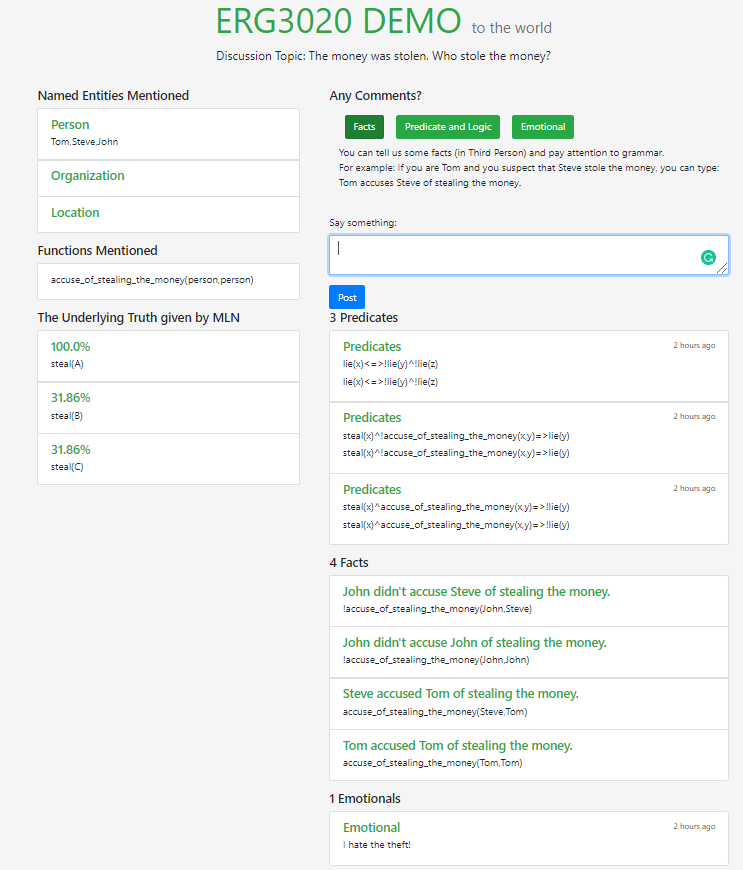
\includegraphics[width=\columnwidth]{Flask.png} 
    \caption[An Screenshot of the website]{An Screenshot of the website} % The text in the square bracket is the caption for the list of figures while the text in the curly brackets is the figure caption
    \end{figure}

we can find that we can input and post comments in a text area. We even can choose the type of the comments. However, if we choose the wrong type, the NLP model will indentify it and change the type into the correct one. All of the comments will be showed below the text area. Also, the names and functions in the comments will be showed in the left sides. The result of the Markov Logic Networks will be showed below them.

\section{The Architecture of Jianfeng Demo}

\subsection{Users Can Post 3 Kinds of Comments}

Difference from traditional social network, here users can choose 3 different columns to post their comments: \textit{Facts, Predicates, Emotional}. 

For \textit{Facts} column, users can post the facts they have mastered. For example, if the user know that \textit{Albert accuses Bob of stealing the final paper}, he or she could type \textit{Albert accuses Bob of stealing the final paper}. To make sure that the facts are valid, citation and source verification features will be added in the future.

\begin{figure}[htb]
    \centering 
    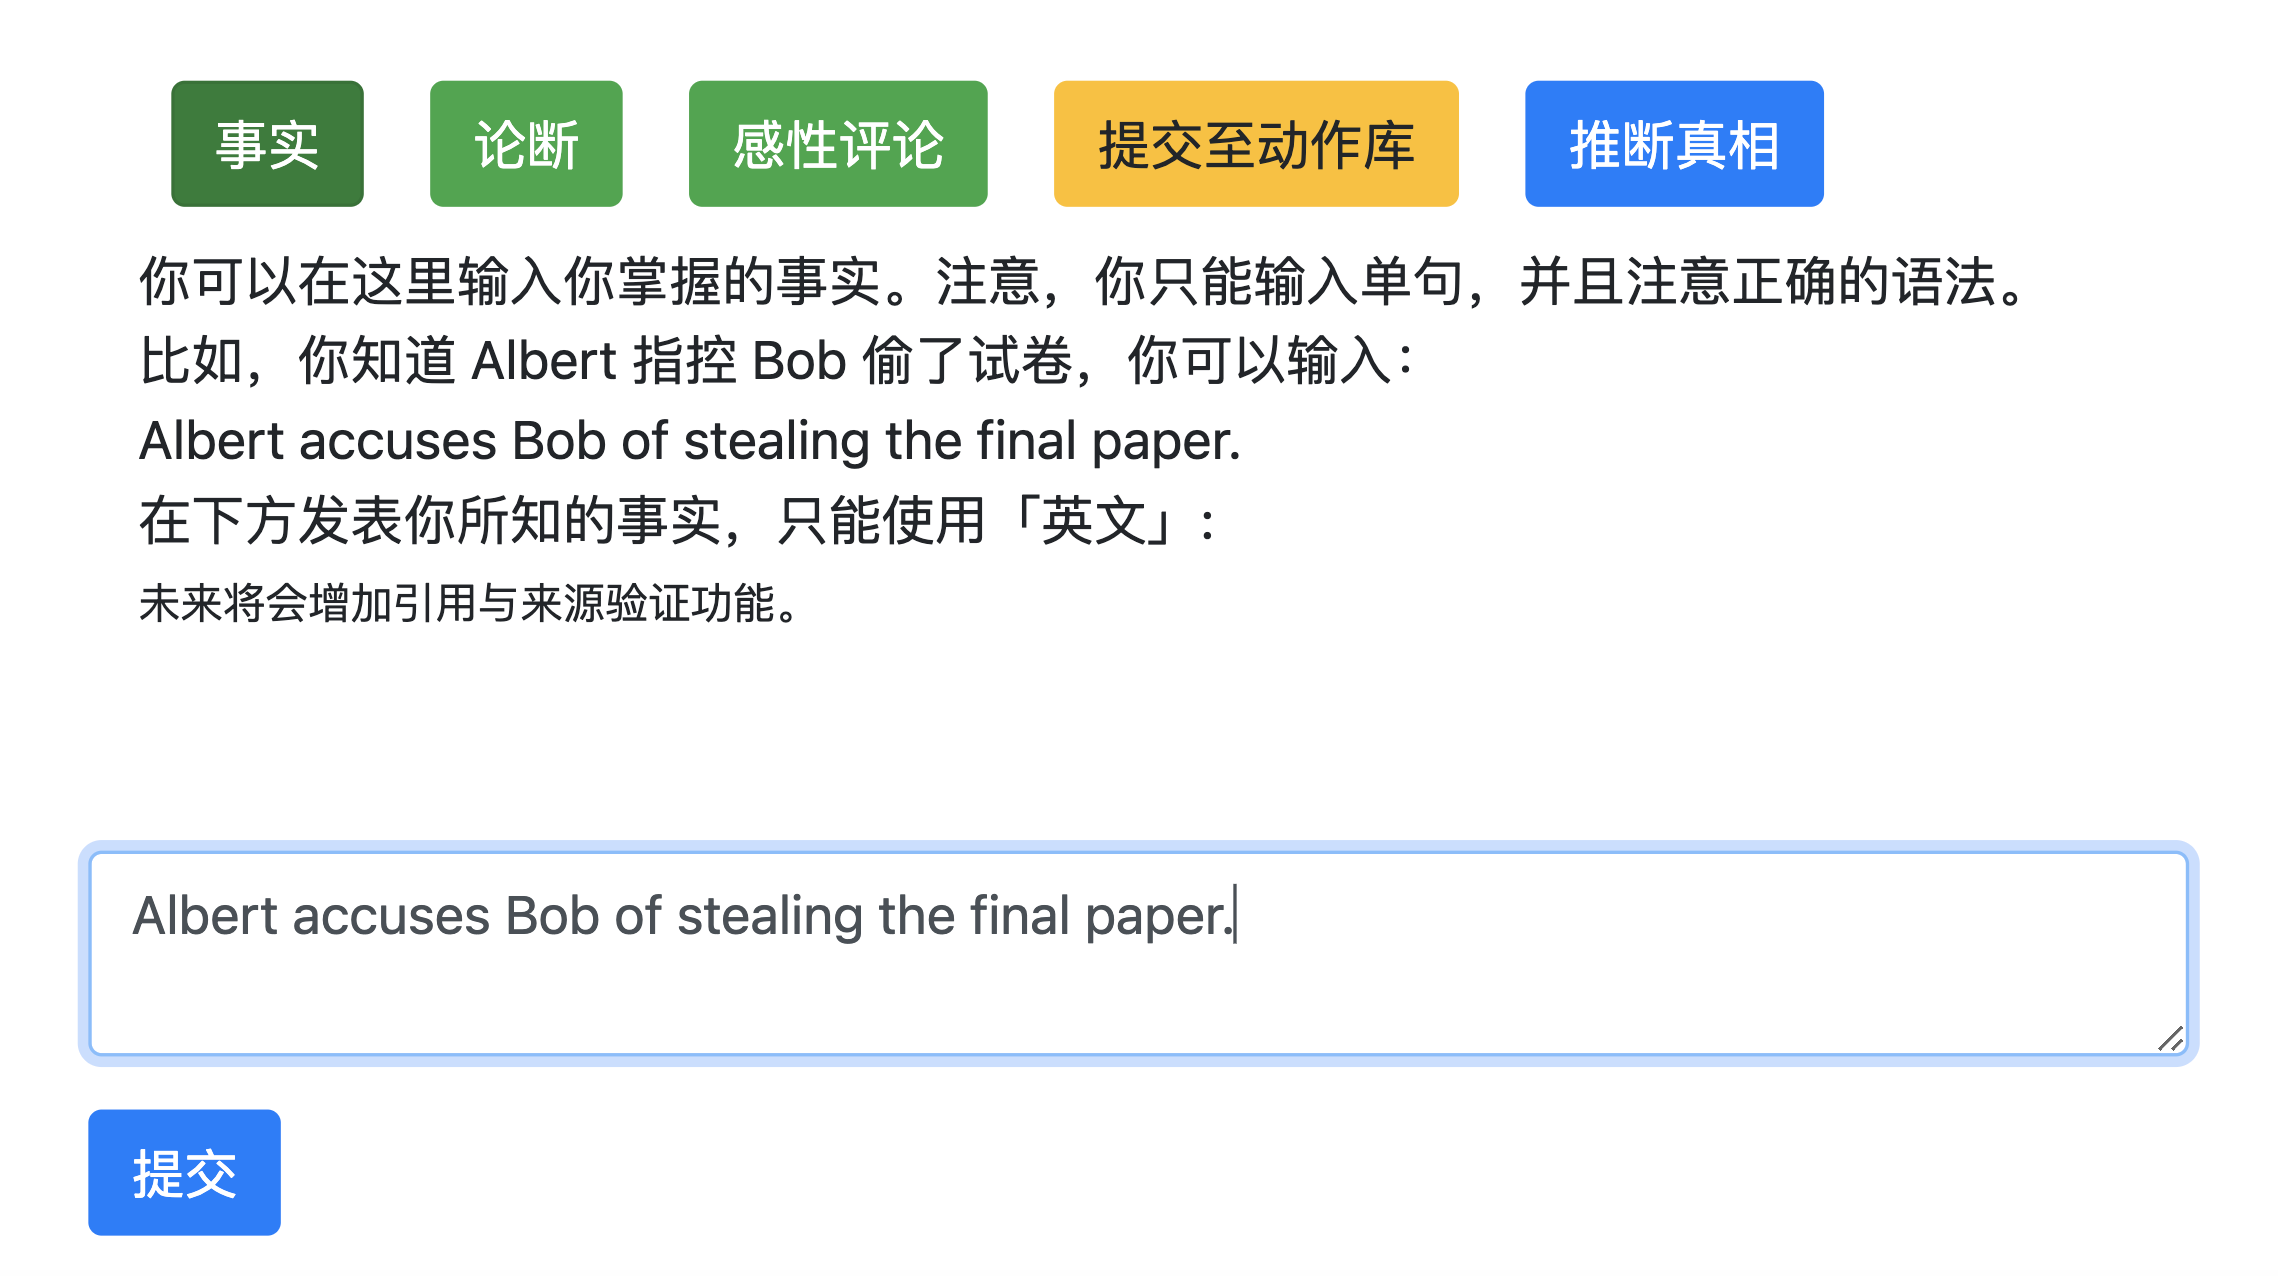
\includegraphics[width=\columnwidth]{arch1.png} 
    \caption[Prompting Users to Post facts]{Prompting Users to Post facts} 
    \end{figure}

For \textit{Predicates} column, users can post their own judgements and theories. These predicates are general and can reveal their thoughts. To make sure the meaning of the logic expression is correct, we only accept First Order Logic expressions. We expect well educated users to post on \textit{Predicates} column. To make this process more smooth, we provide a toolbox for our users. For example, we provide widely used logic operators, function library, undetermined objects.

\begin{figure}[htb]
    \centering 
    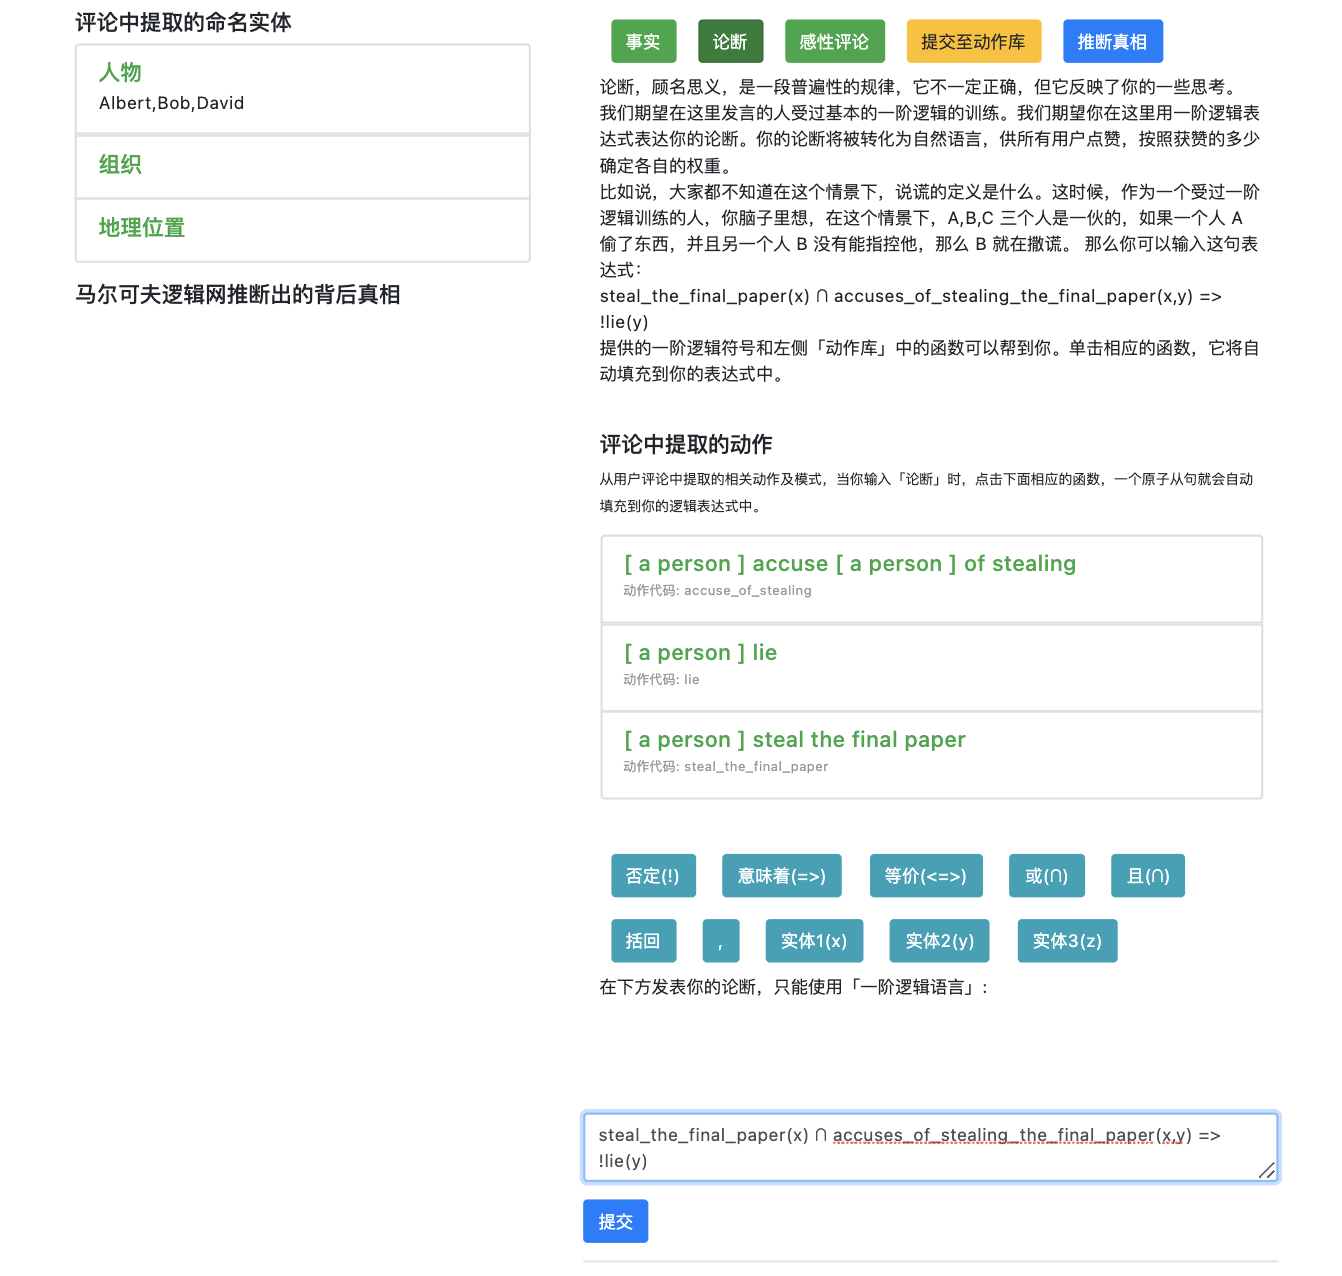
\includegraphics[width=\columnwidth]{arch5.png} 
    \caption[Prompting Users to Post facts]{Prompting Users to Post Facts} 
\end{figure}
    
After users post their \textit{Predicates}, their logic expressions will be stored in our system and we design an algorithm to convert the logic expression into natural language. We display the natural language version of the \textit{Predicates} on the front end, other users can give \textit{likes} to each \textit{Predicates}. We will determine the \textit{weights} of the \textit{Predicates}. The \textit{weights} of each \textit{Predicates} are important in Markov Logic Network, they are the \textit{strength} of constraints.

For \textit{Emotional} column. In this column, users are welcomed to post everything they want. This column is an area for users to post their emotional comments, and if users post emotional comments in \textit{Facts} column, the comments will be transferred to this column because we also design an algorithm to recognize if the comments are really \textit{Facts} or \textit{Predicates}. 


\begin{figure}[htb]
    \centering 
    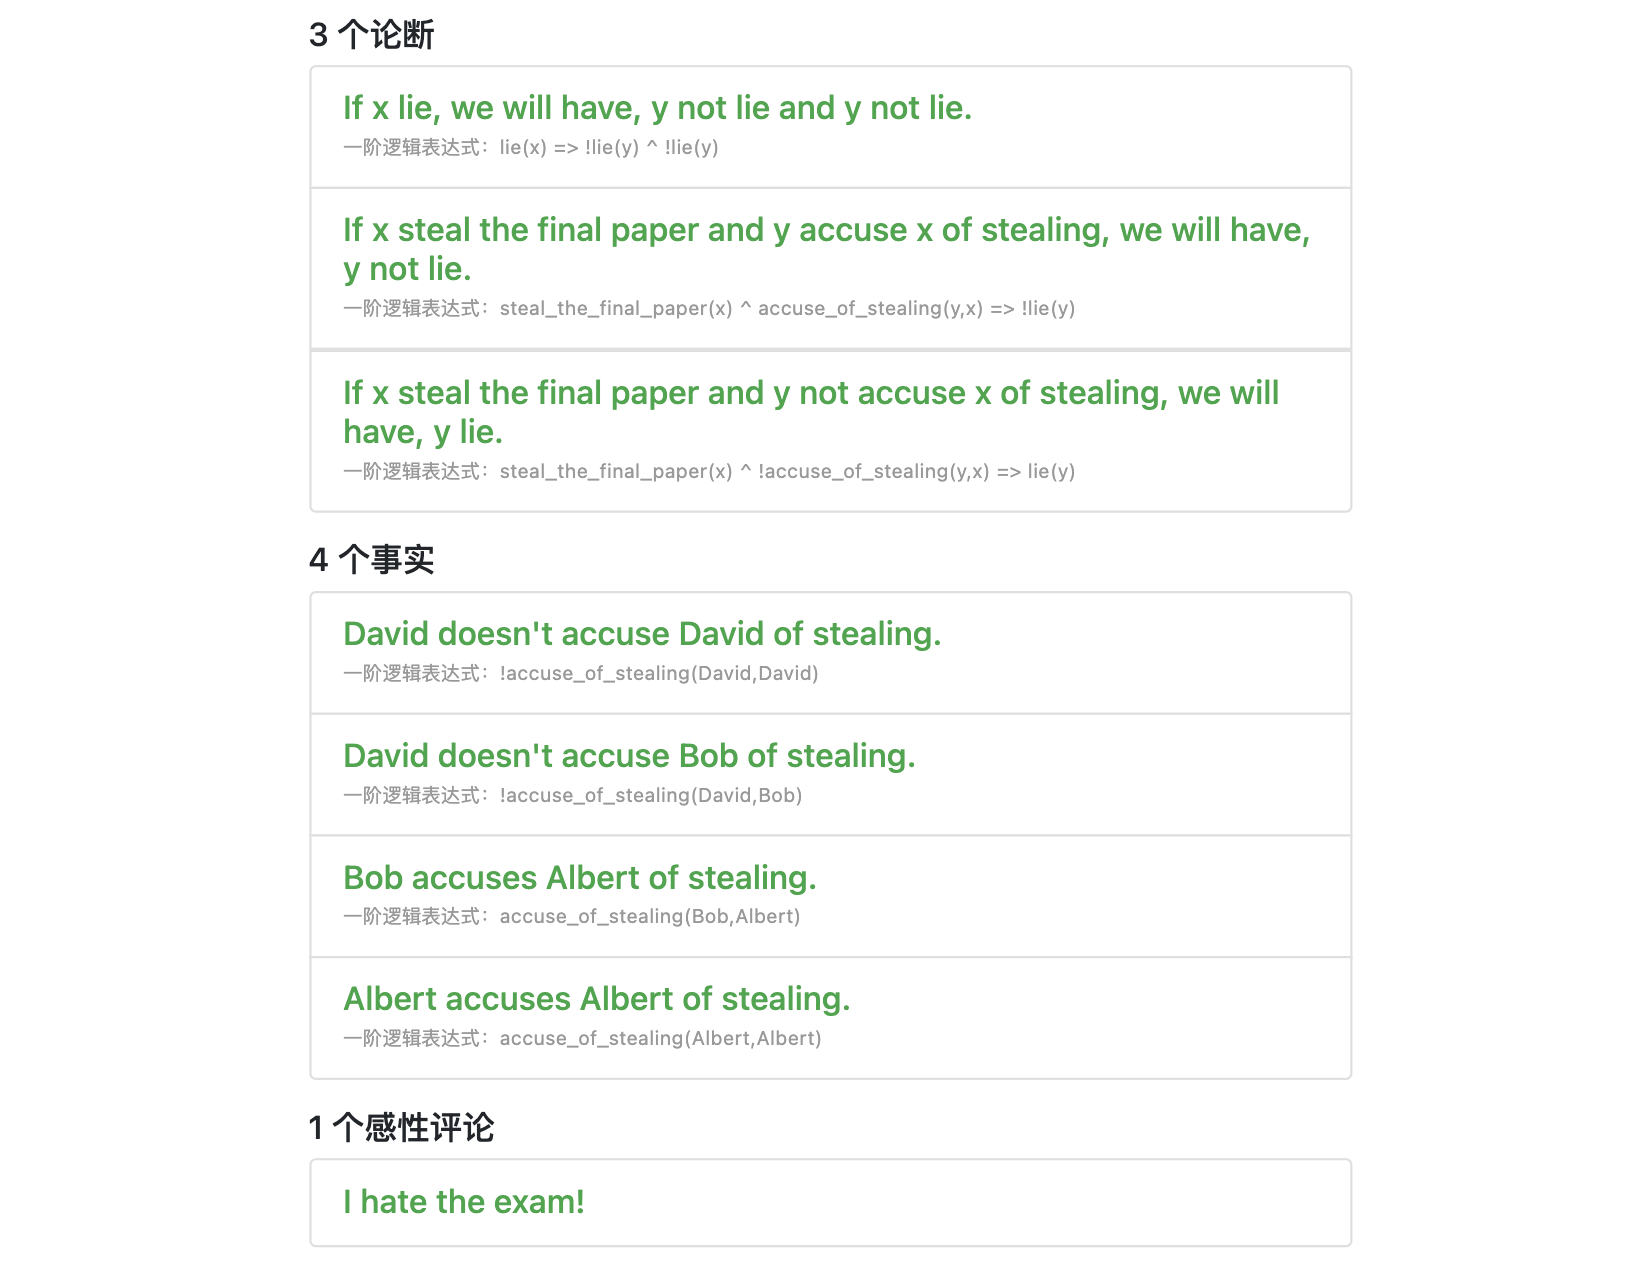
\includegraphics[width=\columnwidth]{arch8.png} 
    \caption[Displaying the Comments on Front End]{Displaying the Comments on Front End} 
    \end{figure}



\subsection{For Less Educated Users}


Jianfeng is desgined to the serve the public, and its users are mainly less educated users. Less educated users accounts for the majority of our users. So, we carefully designed the architecture of Jianfeng. 

\begin{figure}[htb]
    \centering 
    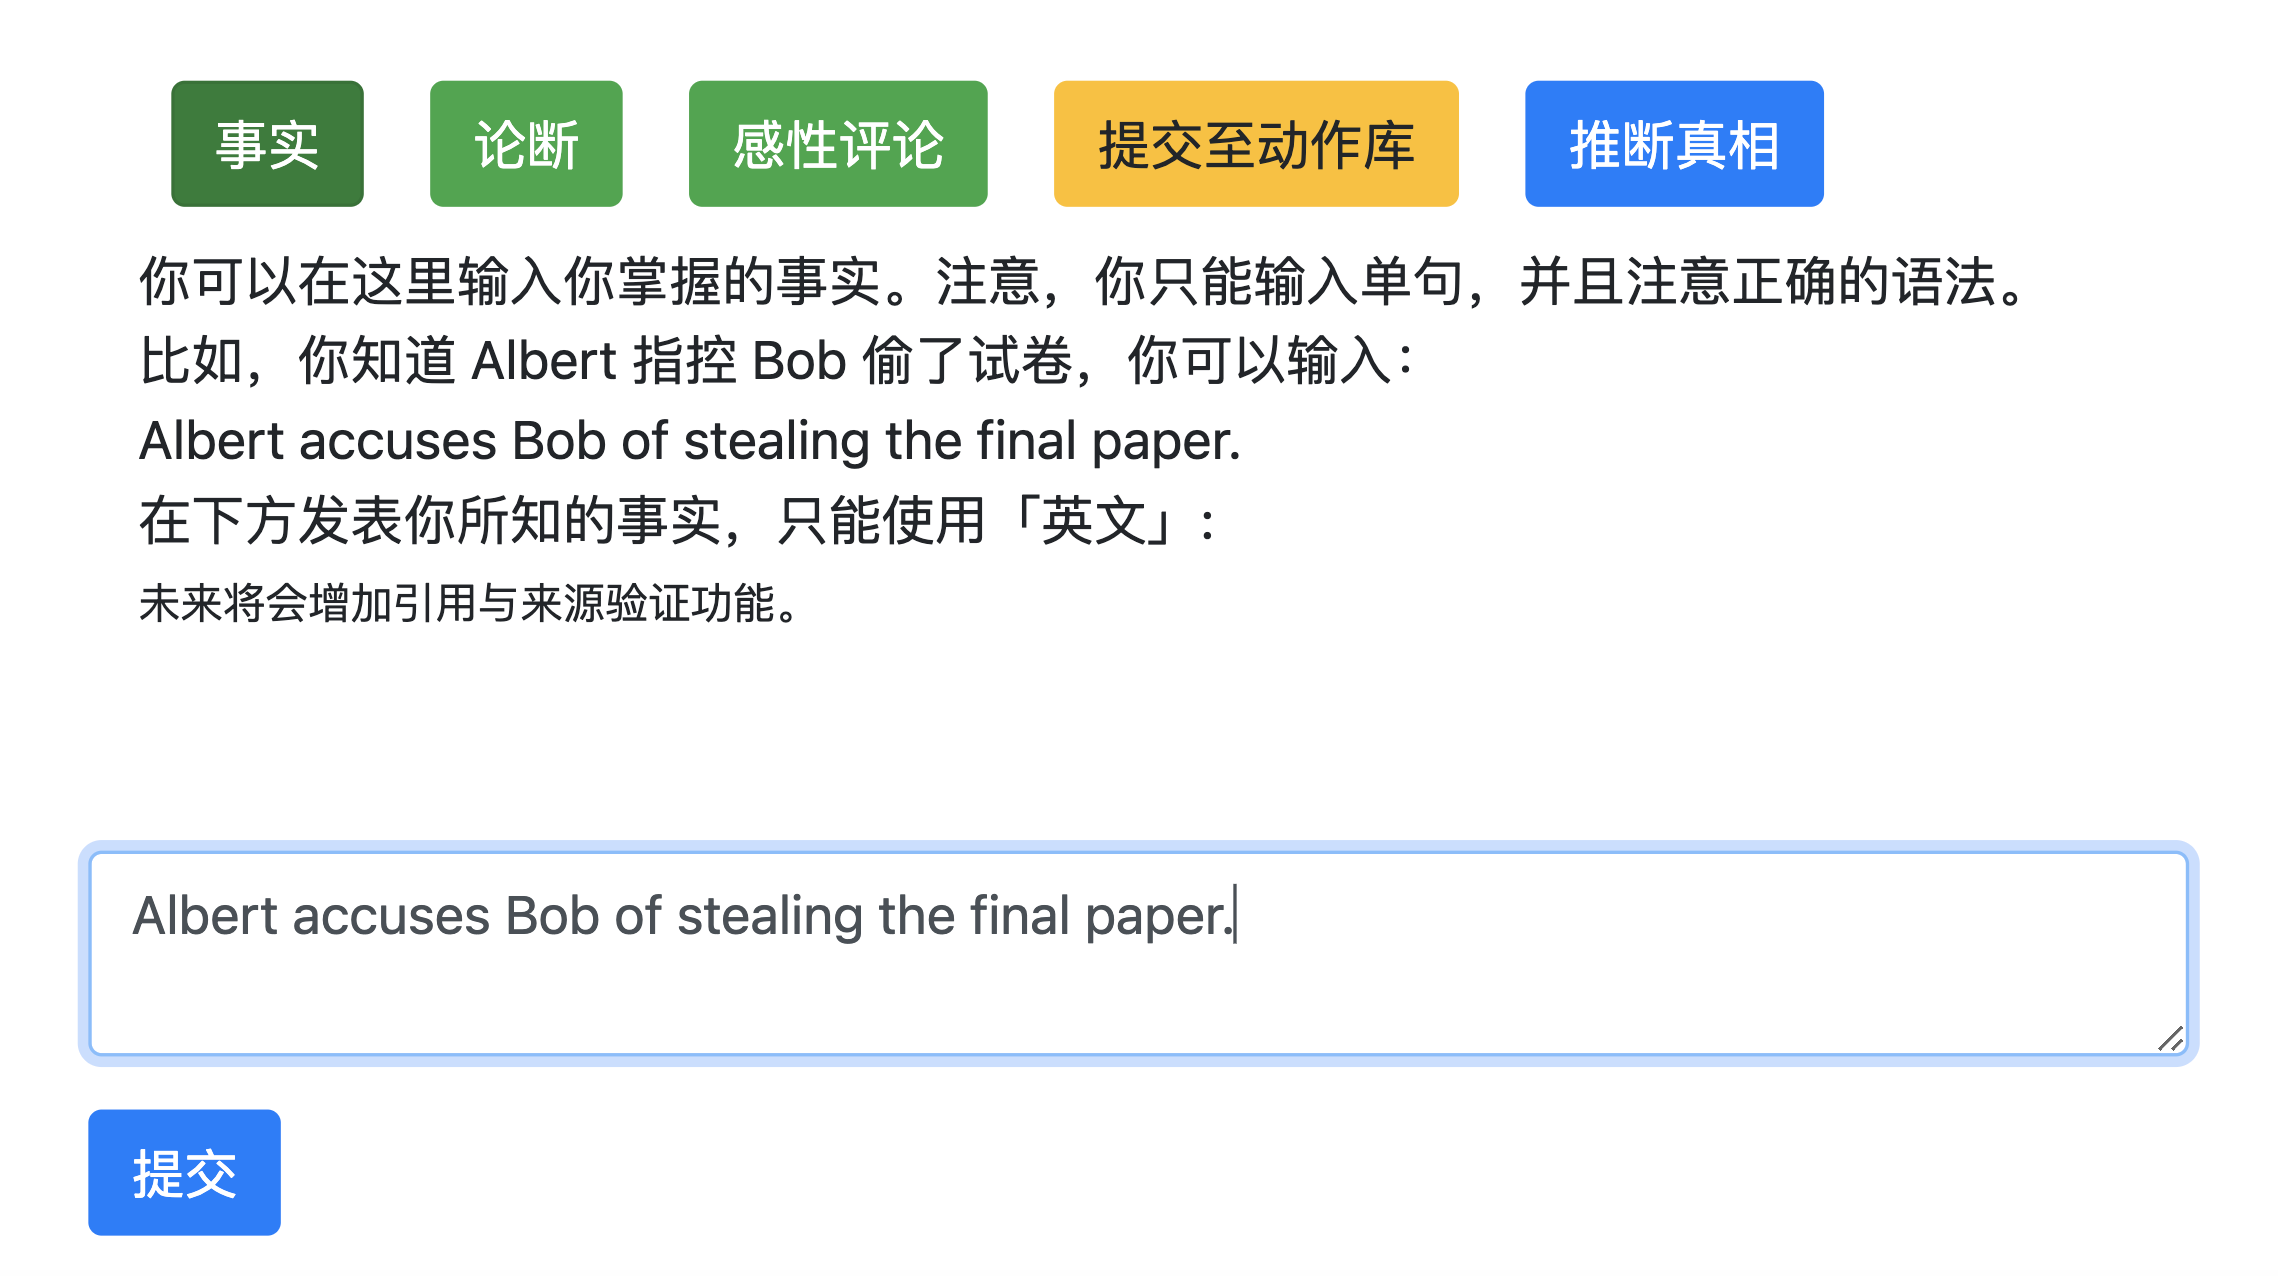
\includegraphics[width=\columnwidth]{fact_usr.png} 
    \caption[Prompting User to Commit Facts]{Prompting User to Commit Facts} 
    \end{figure}

Less educated users can post the facts they know just by typing English sentences. 


The facts in natural language will be processed by AllenNLP Open Information Extraction module [cite: https://demo.allennlp.org/open-information-extraction] first. The result given by AllenNLP is as follows:

\begin{figure}[htb]
    \centering 
    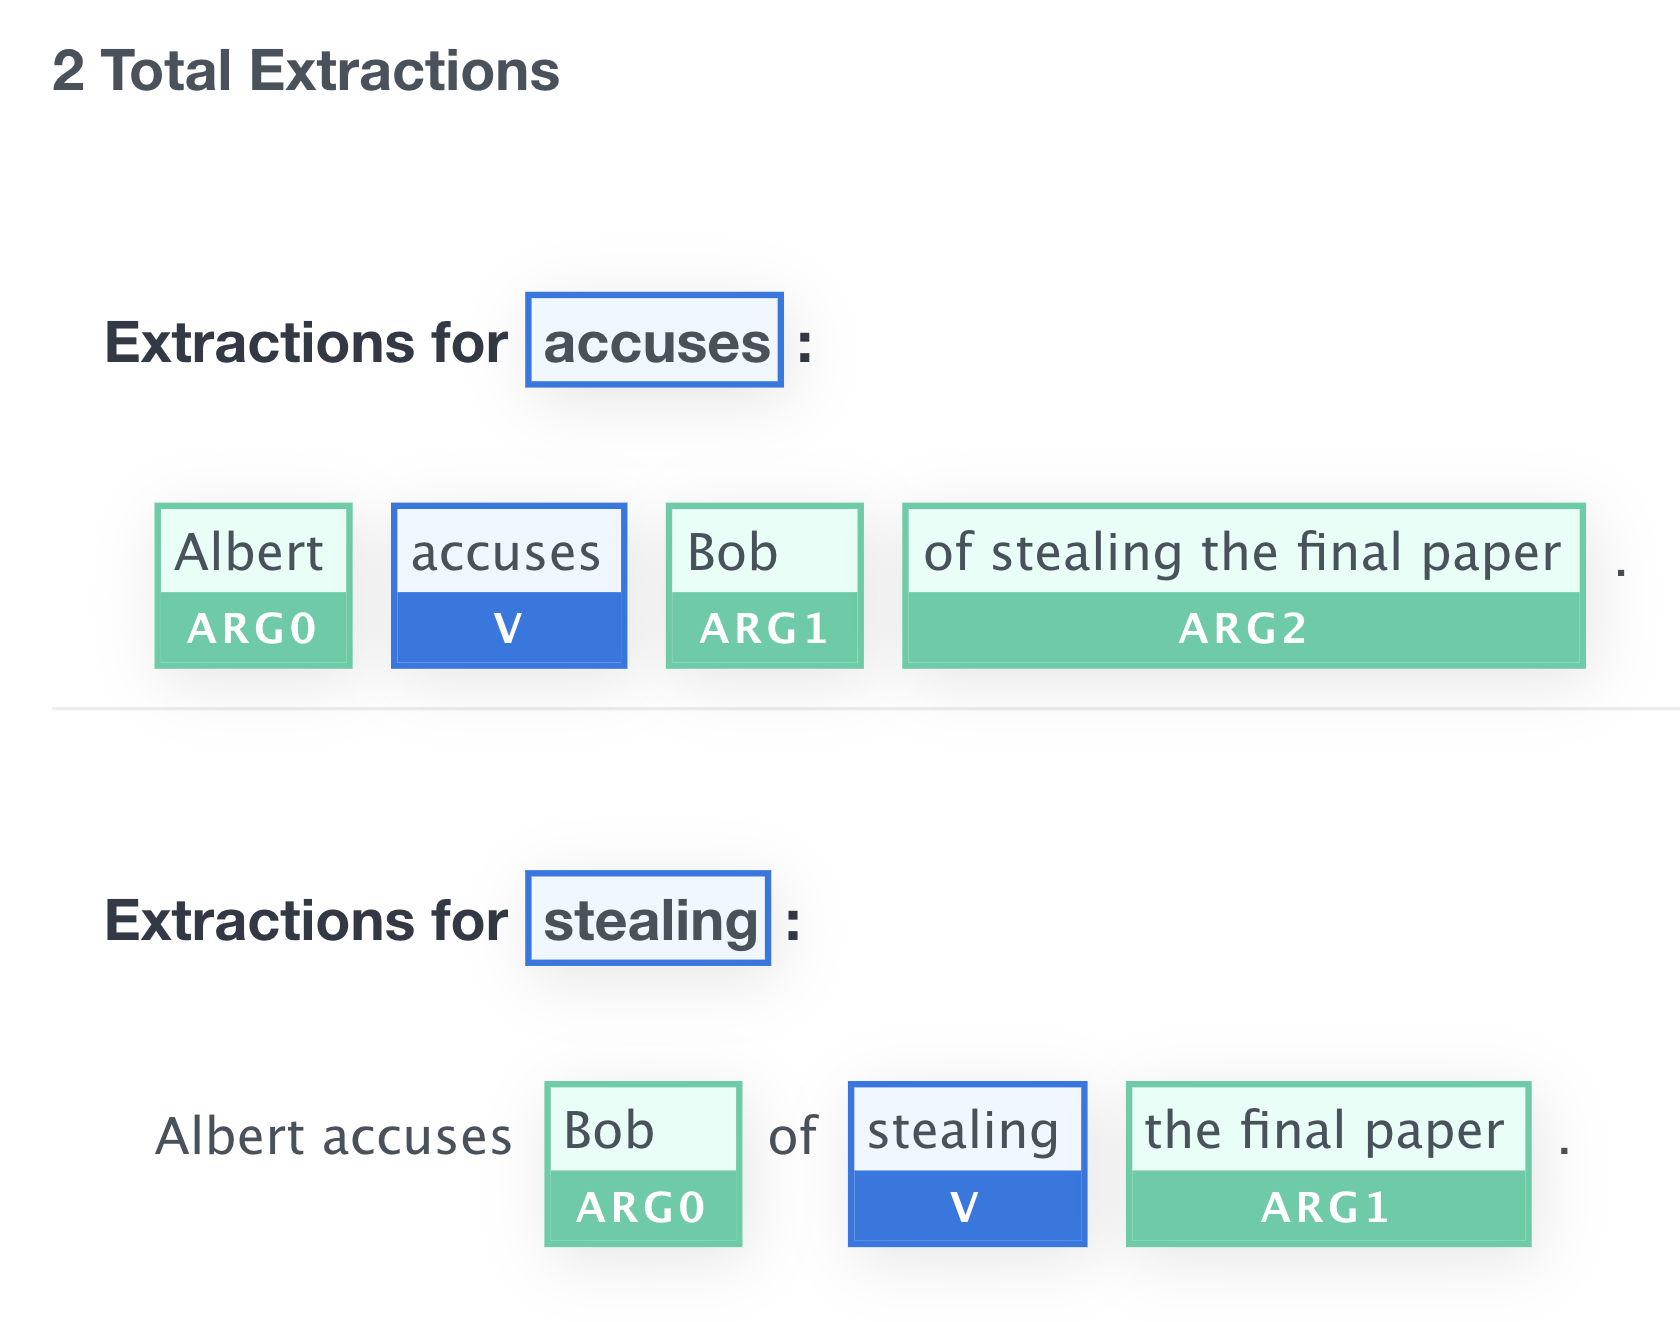
\includegraphics[width=\columnwidth]{nlp1.png} 
    \caption[Primary Result Given by AllenNLP Open Information Extraction module]{Primary Result Given by AllenNLP Open Information Extraction module} 
    \end{figure}

AllenNLP gives multiple results of one single sentence, and we want to find one that can best model that sentence. We choose the verb which can recognize most words as its arguments. We call that verb the best verb of that sentence. 

\begin{figure}[htb]
    \centering 
    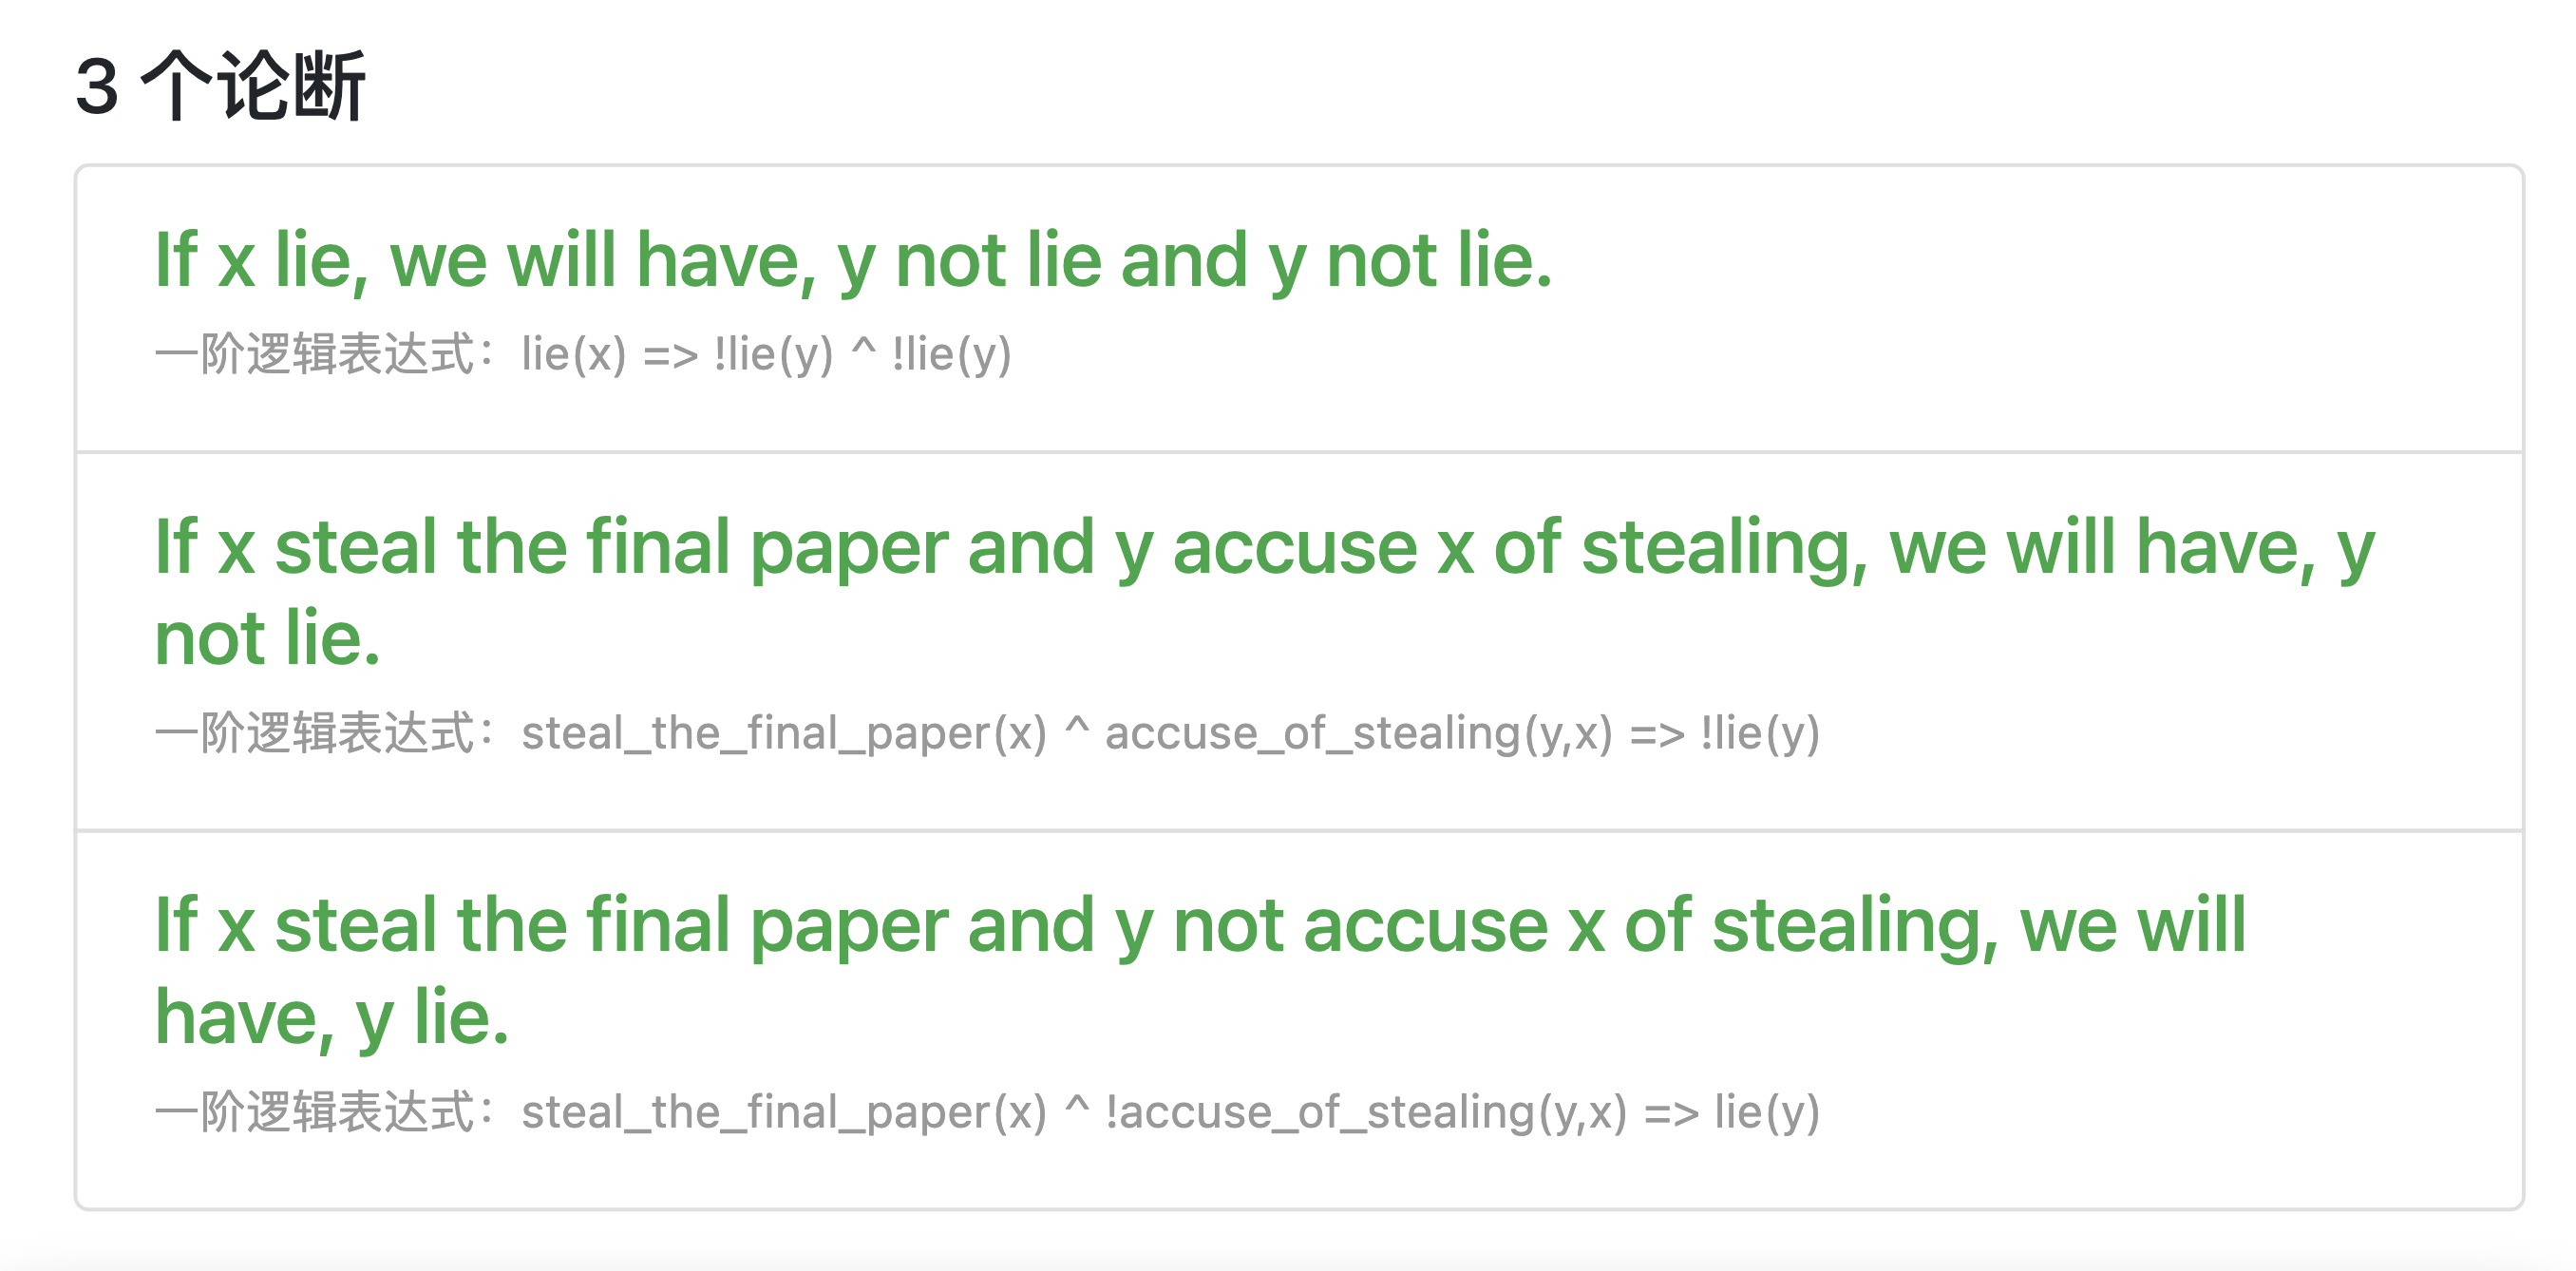
\includegraphics[width=\columnwidth]{nlp3.png} 
    \caption[Natural Language Converted]{Natural Language Converted} 
    \end{figure}
    
Then we consider the best verb and its arguments. For example, we input the sentence \textit{Albert accuses Bob of stealing the final paper.}, and the output has two possible results: \textit{accuse} and \textit{steal}. Then we choose \textit{accuse} as our best verb because it can utilize 3 components as its arguments.

The next step is to utilize AllenNLP Named Entity Recognition module to check each argument to see if it is a named entity, for example, \textit{Albert} and \textit{Bob} will be recognized as \textit{Person}; \textit{of stealing the final paper} will be not recognized. Then, we append \textit{of stealing the final paper} to the verb and only keep \textit{Albert} and \textit{Bob} as arguments. Then we can construct the function $accuses\_of\_stealing\_the\_final\_paper$ with two input arguments \textit{ARG0: Person} and \textit{ARG1: Person}. Here we can express this fact as $accuse\_of\_stealing\_the\_final\_paper \left(Albert, Bob\right)$. 

After we extract the function mode, we will first append this function to the library, in Jianfeng Demo, we call it \textit{The Actions Extracted From User Comments}. But in consideration the experience of less educated users, we design an algorithm to convert functions into natural language expressions. For example, if the user submitted \textit{Albert accuses Bob of stealing the money}, we will first extract the function mode and store it into \textit{action library} and then compile it into natural language expression, then display it on the front end.

Less educated users can also post emotional comments. We give them a choice to post whatever they want. Users can choose \textit{Emotional} module to post their comments. 

We also design an algorithm to convert First Order Logic expression into natural language. Because some well educated users can post First Order Logic expressions and complex expressions, it is usually hard to read for less educated users. It is necessary to convert every piece of logic expression into natural language. And we realize this function in Jianfeng demo.




\subsection{Cumulative Action Library}

Jianfeng Demo will continuously collect actions submitted by users. Once user post a fact containing valid information, we will automatically analyze the action mode in this sentence. Then it will be stored in our \textit{Action Library} and we will convert it into a form which can be easily understood by users and then display them on the front end.

Users can submit new \textit{action modes} to \textit{Action Library}. We provide a column for users to submit new mode. Users only need to provide a sentence in this dialogue, and they don't need think about the details. We will automatically analyze the sentence and extract the \textit{action mode} in this sentence. 

Besides, the \textit{Action Library} in Jianfeng Demo is cumulative. We will keep all the \textit{action modes} in our database, and once a new event emerges, users can conveniently use previously defined \textit{action modes}.

We expect in a few months, we can collect all the possible action modes in human language. In that case, we will provide more complete toolbox for educated users who have a good command of First Order Logic to composite their predicates. 

Furthermore, the \textit{action modes} in consideration within an event comply with the following conditions:

1. That \textit{action mode} is mentioned in \textit{Facts}.

2. That \textit{action mode} is mentioned in \textit{Predicates}.

\textit{Action modes} satisfy the above conditions will be declared in Markov Logic Network inference process. 

\begin{figure}[htb]
    \centering 
    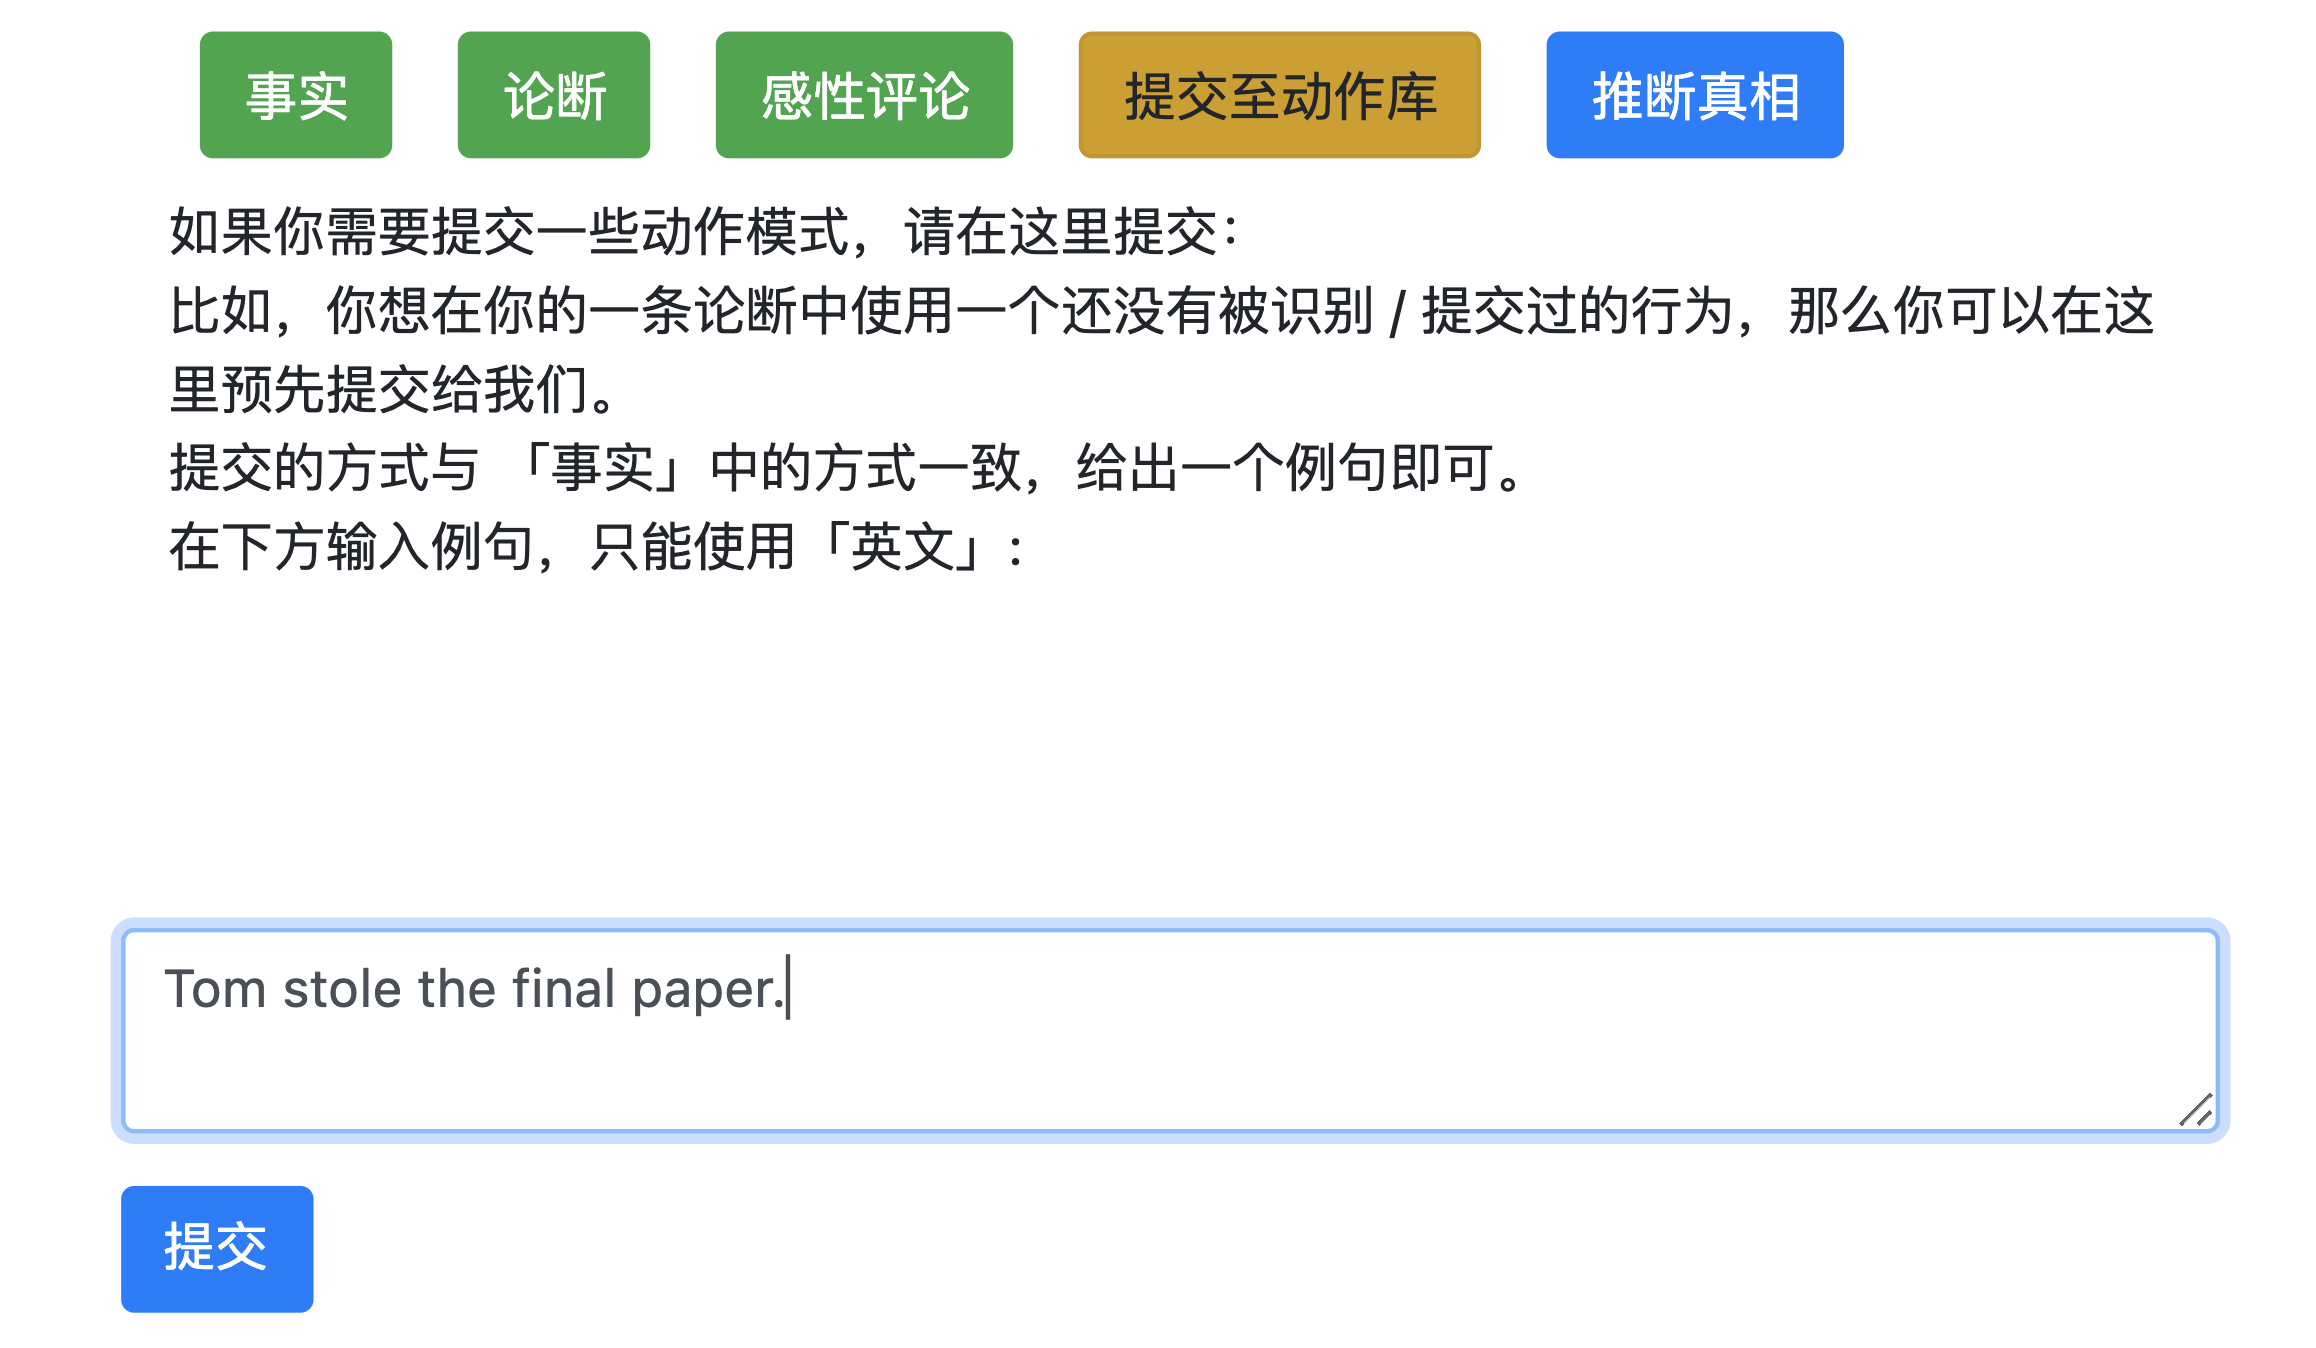
\includegraphics[width=\columnwidth]{arch9.png} 
    \caption[Action Mode Submission Dialog]{Action Mode Submission Dialog} 
    \end{figure}

\subsection{Cumulating Predicate Library} 


\begin{figure}[htb]
    \centering 
    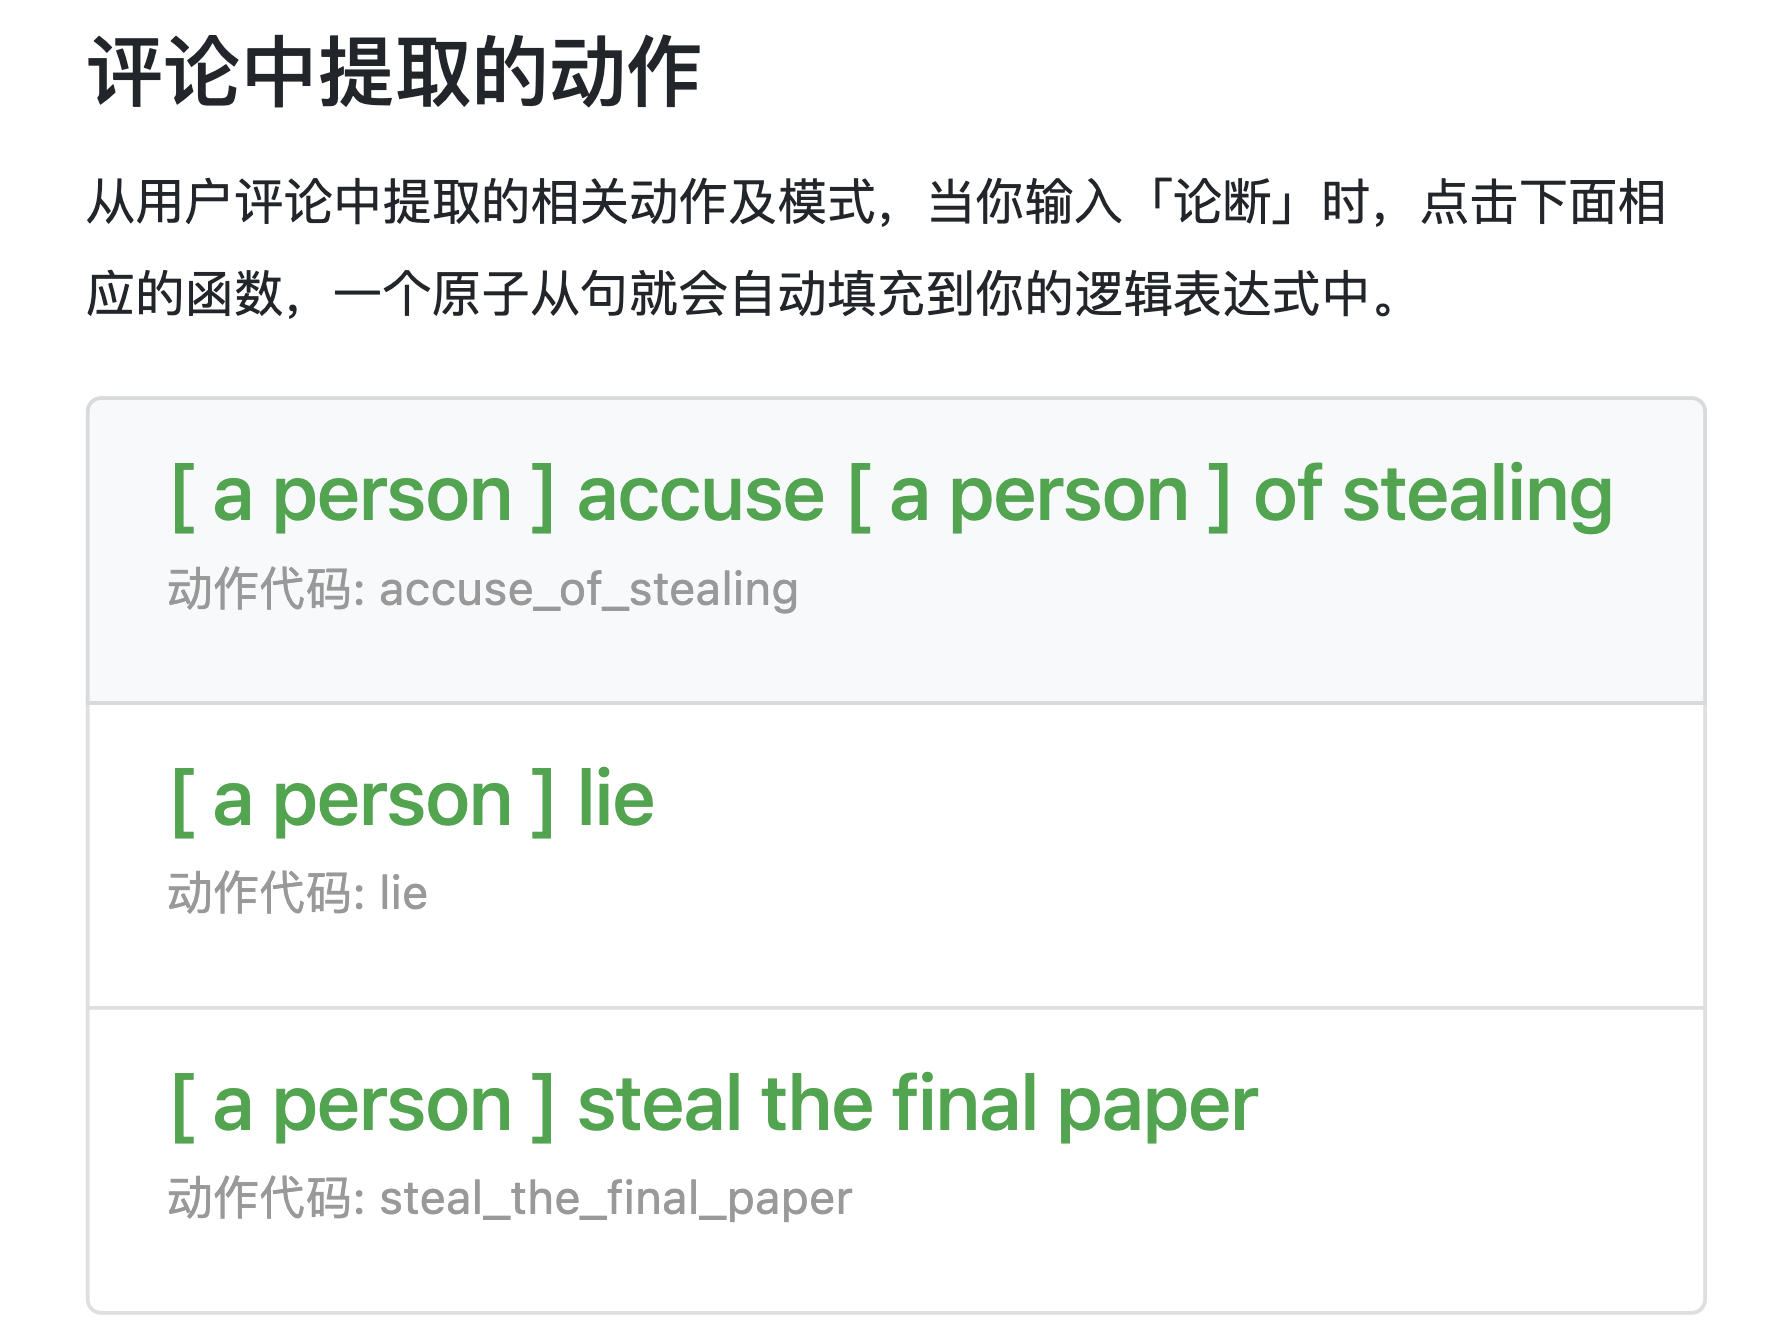
\includegraphics[width=\columnwidth]{nlp2.png} 
    \caption[Natural Language Expression of Action Library]{Natural Language Expression of Action Library} 
    \end{figure}

\clearpage

\section{Example}
Here we show a example with full steps of the usage of the demo.

We first input some facts:
$$
facts.jpg
$$

Then we input some predicates and logic:
$$
predicates and logic.jpg
$$

Also we can input some emotionals (Whichever the type we choose they will be shown as the emotionals finally):
$$
emotionals.jpg
$$

Now, we can find that all of the names and functions appeared in the comments are clearly showed in the left side:

$$
appear.jpg
$$

We click the button of running the markov logic networks and find that the result is showed below in the form of probabilities:
$$
result.jpg
$$

\section{Conclusion and further development}

\section{Introduction}

A statement requiring citation.

\lipsum[1-3] % Dummy text

Some mathematics in the text: $\cos\pi=-1$ and $\alpha$.
 
%----------------------------------------------------------------------------------------
%	METHODS
%----------------------------------------------------------------------------------------

\section{Methods}

\lipsum[5] % Dummy text

\begin{enumerate}[noitemsep] % [noitemsep] removes whitespace between the items for a compact look
\item First item in a list
\item Second item in a list
\item Third item in a list
\end{enumerate}

%------------------------------------------------

\subsection{Paragraphs}

\lipsum[6] % Dummy text

\paragraph{Paragraph Description} \lipsum[7] % Dummy text

\paragraph{Different Paragraph Description} \lipsum[8] % Dummy text

%------------------------------------------------

\subsection{Math}

\lipsum[4] % Dummy text

\begin{equation}
\cos^3 \theta =\frac{1}{4}\cos\theta+\frac{3}{4}\cos 3\theta
\label{eq:refname2}
\end{equation}

\lipsum[5] % Dummy text

\begin{definition}[Gauss] 
To a mathematician it is obvious that
$\int_{-\infty}^{+\infty}
e^{-x^2}\,dx=\sqrt{\pi}$. 
\end{definition} 

\begin{theorem}[Pythagoras]
The square of the hypotenuse (the side opposite the right angle) is equal to the sum of the squares of the other two sides.
\end{theorem}

\begin{proof} 
We have that $\log(1)^2 = 2\log(1)$.
But we also have that $\log(-1)^2=\log(1)=0$.
Then $2\log(-1)=0$, from which the proof.
\end{proof}

%----------------------------------------------------------------------------------------
%	RESULTS AND DISCUSSION
%----------------------------------------------------------------------------------------

\section{Results and Discussion}

Reference to Figure~\vref{fig:gallery}. % The \vref command specifies the location of the reference

\begin{figure}[tb]
\centering 
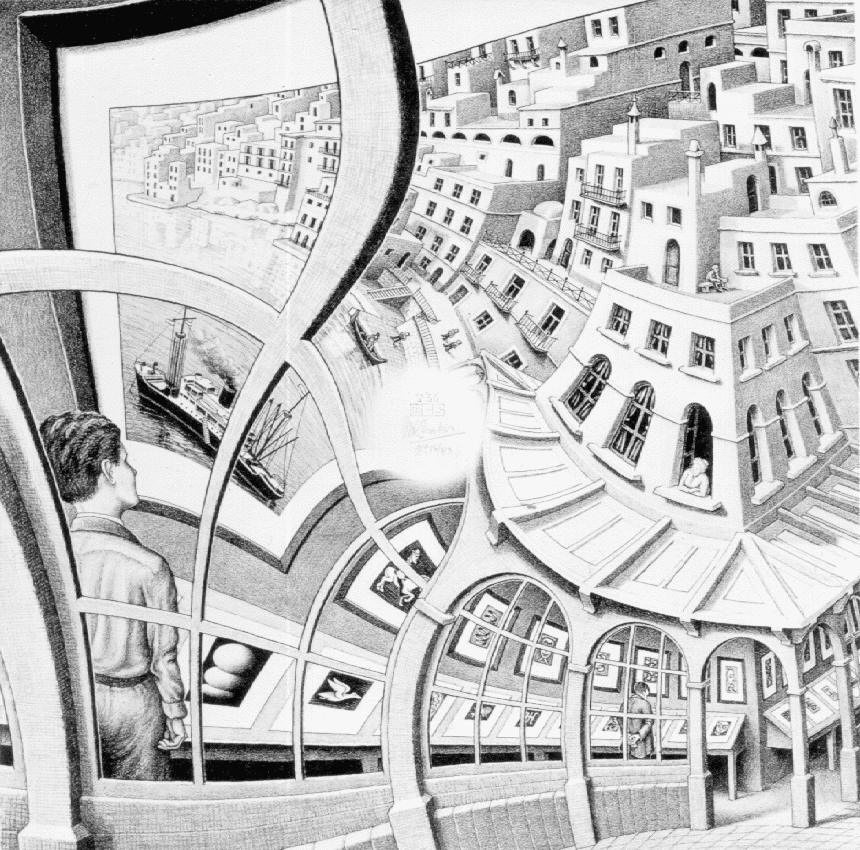
\includegraphics[width=0.5\columnwidth]{GalleriaStampe} 
\caption[An example of a floating figure]{An example of a floating figure (a reproduction from the \emph{Gallery of prints}, M.~Escher,\index{Escher, M.~C.} from \url{http://www.mcescher.com/}).} % The text in the square bracket is the caption for the list of figures while the text in the curly brackets is the figure caption
\label{fig:gallery} 
\end{figure}

\lipsum[10] % Dummy text

%------------------------------------------------

\subsection{Subsection}

\lipsum[11] % Dummy text

\subsubsection{Subsubsection}

\lipsum[12] % Dummy text

\begin{description}
\item[Word] Definition
\item[Concept] Explanation
\item[Idea] Text
\end{description}

\lipsum[12] % Dummy text

\begin{itemize}[noitemsep] % [noitemsep] removes whitespace between the items for a compact look
\item First item in a list
\item Second item in a list
\item Third item in a list
\end{itemize}

\subsubsection{Table}

\lipsum[13] % Dummy text

\begin{table}[hbt]
\caption{Table of Grades}
\centering
\begin{tabular}{llr}
\toprule
\multicolumn{2}{c}{Name} \\
\cmidrule(r){1-2}
First name & Last Name & Grade \\
\midrule
John & Doe & $7.5$ \\
Richard & Miles & $2$ \\
\bottomrule
\end{tabular}
\label{tab:label}
\end{table}

Reference to Table~\vref{tab:label}. % The \vref command specifies the location of the reference

%------------------------------------------------

\subsection{Figure Composed of Subfigures}

Reference the figure composed of multiple subfigures as Figure~\vref{fig:esempio}. Reference one of the subfigures as Figure~\vref{fig:ipsum}. % The \vref command specifies the location of the reference

\lipsum[15-18] % Dummy text

\begin{figure}[tb]
\centering
\subfloat[A city market.]{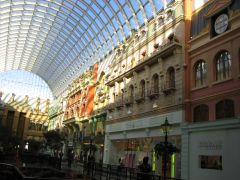
\includegraphics[width=.45\columnwidth]{Lorem}} \quad
\subfloat[Forest landscape.]{
\includegraphics[width=.45\columnwidth]{Ipsum}\label{fig:ipsum}} \\
\subfloat[Mountain landscape.]{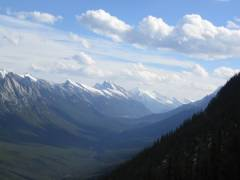
\includegraphics[width=.45\columnwidth]{Dolor}} \quad
\subfloat[A tile decoration.]{
\includegraphics[width=.45\columnwidth]{Sit}}
\caption[A number of pictures.]{A number of pictures with no common theme.} % The text in the square bracket is the caption for the list of figures while the text in the curly brackets is the figure caption
\label{fig:esempio}
\end{figure}

%----------------------------------------------------------------------------------------
%	BIBLIOGRAPHY
%----------------------------------------------------------------------------------------

\renewcommand{\refname}{\spacedlowsmallcaps{References}} % For modifying the bibliography heading


\clearpage
\bibliographystyle{unsrt}

\bibliography{references.bib} % The file containing the bibliography

%----------------------------------------------------------------------------------------
\clearpage
\appendix
\section{A guidence to running code}
First we have to make sure the working director of the ternimal is the code folder. Then we type the below codes:
\begin{lstlisting}
    pip install -r requirements.txt
\end{lstlisting}
Then we can find that all the requirements are installed. The next steps are to run the flask app. 
\begin{lstlisting}
    $env:FLASK_APP = "sayhello"
\end{lstlisting}
And then
\begin{lstlisting}
    flask run --host 127.0.0.1 -p 80
\end{lstlisting}
Therefore, the flask app is run and we can see the website.
\end{document}
